\documentclass{article}

\usepackage{graphicx}
\usepackage{tikz}
\usepackage{tikzsymbols}
\usetikzlibrary{calc,patterns,shapes.geometric}
\pagestyle{empty}
\usepackage[margin=0pt]{geometry}
\geometry{papersize={14in,12in}}

\def\centerarc[#1](#2)(#3:#4:#5){\draw[#1] ($(#2)+({#5*cos(#3)},{#5*sin(#3)})$) arc (#3:#4:#5);}

\begin{document}
	\begin{figure}
		\centering
		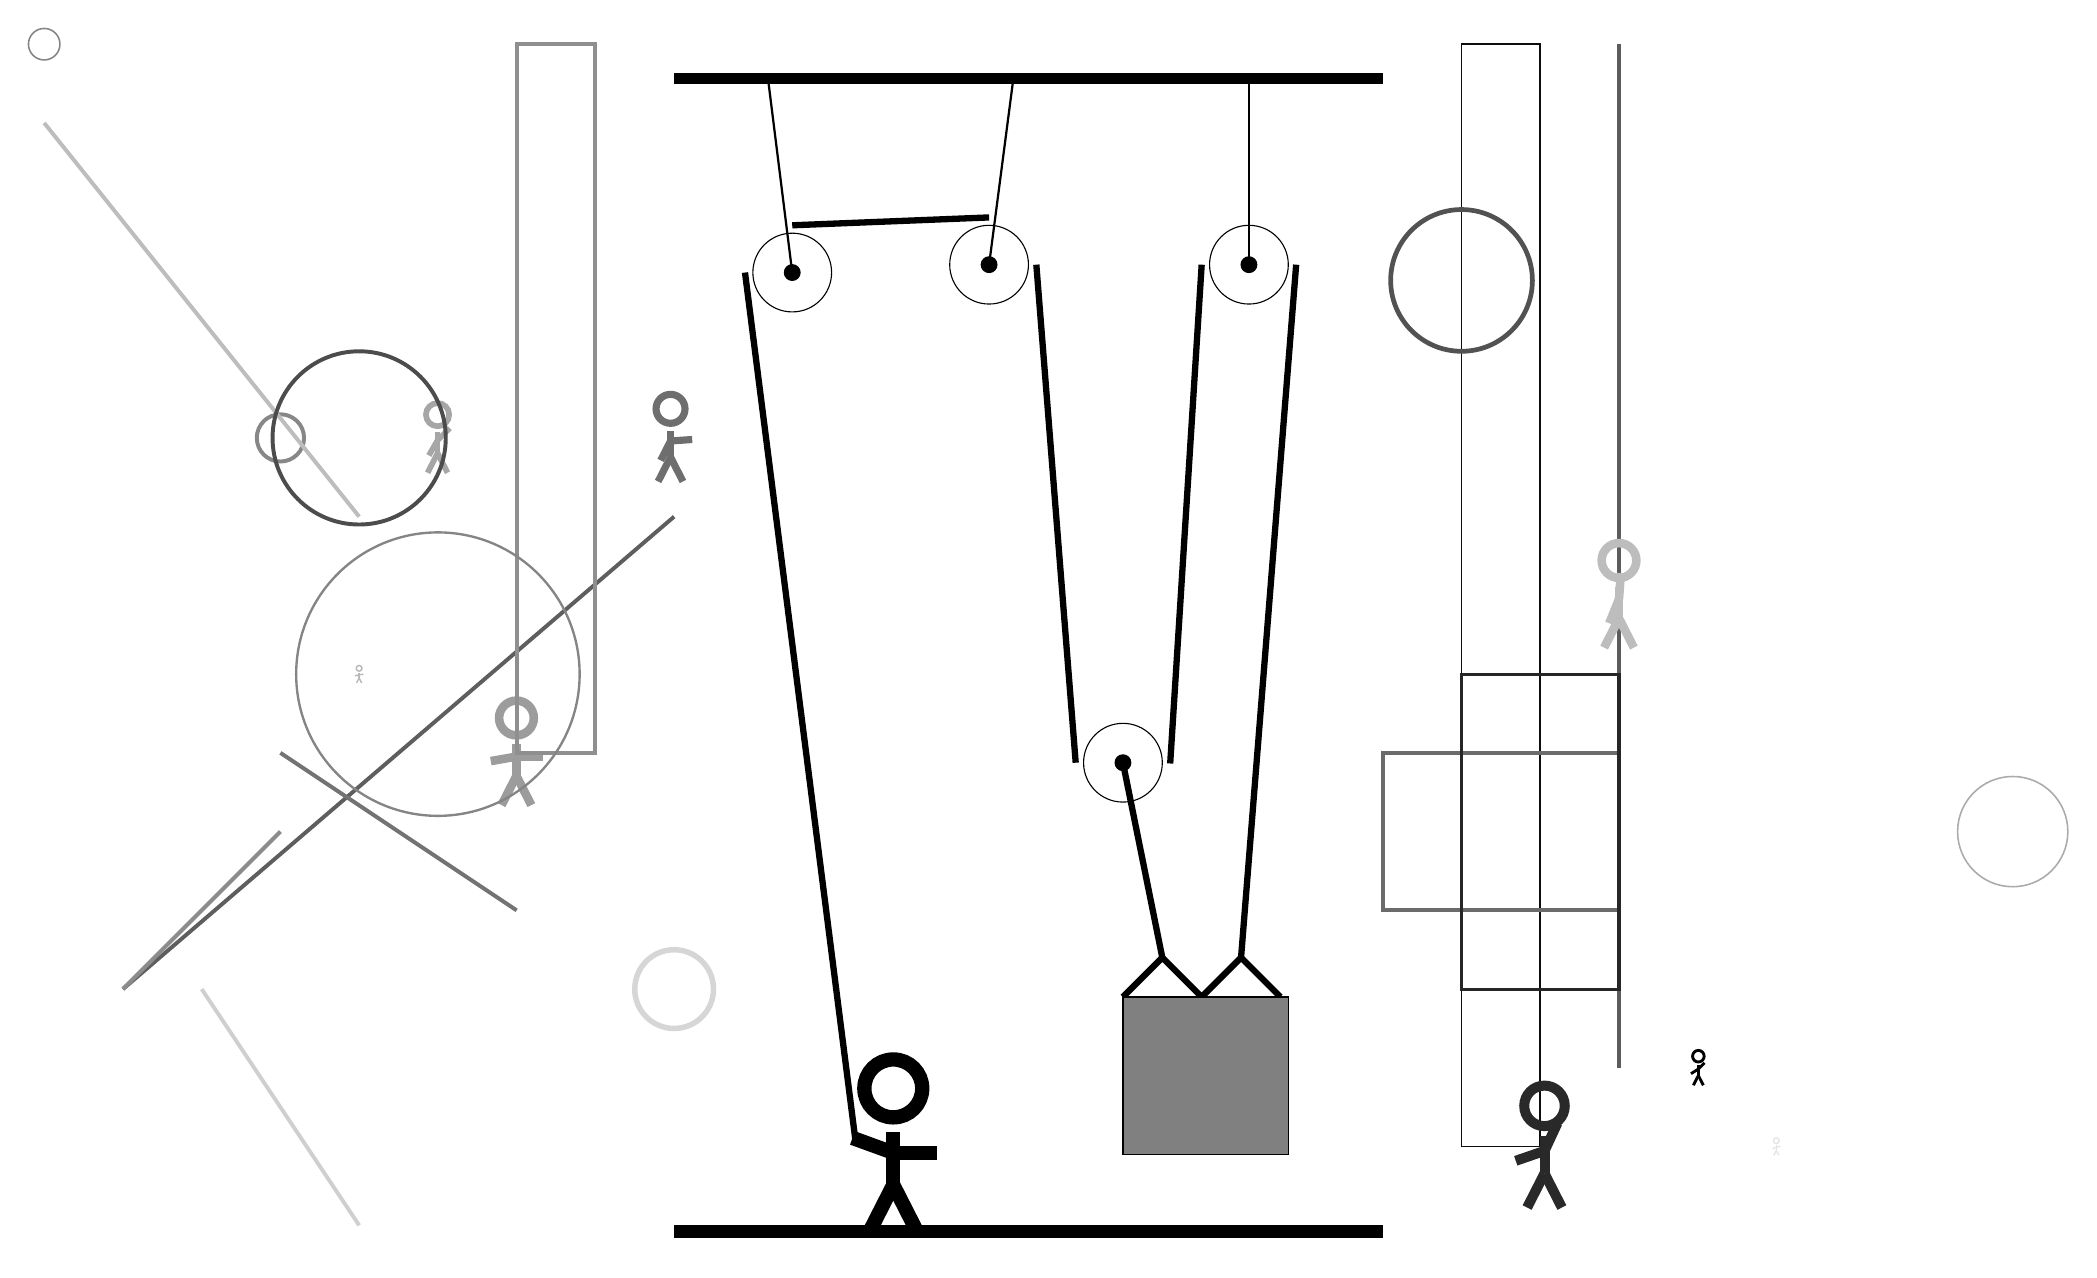
\begin{tikzpicture}
			%%%%% START %%%%%
			
			\draw[fill=black] (-3, 11.5) rectangle (6, 11.625);
			
			\draw (1, 9.2) circle (0.5);
			\draw[fill=black] (1, 9.2) circle (0.1);
			\draw[thick] (1, 9.2) -- (1.3, 11.5);
			
			\draw (4.3, 9.2) circle (0.5);
			\draw[fill=black] (4.3, 9.2) circle (0.1);
			\draw[thick] (4.3, 9.2) -- (4.3, 11.5);
			
			\draw (2.7, 2.875) circle (0.5);
			\draw[fill=black] (2.7, 2.875) circle (0.1);
			
			\draw[line width=0.8mm]  (2.7, -0.1) -- (3.2, 0.4) -- (3.7, -0.1) -- (4.2, 0.4) -- (4.7, -0.1);
			\draw[fill=black!50] (2.7, -0.1) rectangle (4.8, -2.1);
			
			\draw (-1.5, 9.1) circle (0.5);
			\draw[fill=black] (-1.5, 9.1) circle (0.1);
			\draw[thick] (-1.5, 9.1) -- (-1.8, 11.5);
			
			\draw[line width=0.8mm](-0.7, -1.9) --  (-2.1, 9.1);
			\centerarc[line width=0.8mm](-1.5, 9.1)(90:180:0.6);
			\draw[line width=0.8mm](-1.5, 9.7) -- (1, 9.8);
			\centerarc[line width=0.8mm](1, 9.2)(0:90:0.6);
			\draw[line width=0.8mm](1.6, 9.2) -- (2.1, 2.875);
			\centerarc[line width=0.8mm](2.7, 2.875)(180:370:0.6);
			\draw[line width=0.8mm] (3.3, 2.865) -- (3.7, 9.2);
			\centerarc[line width=0.8mm](4.3, 9.2)(0:180:0.6);
			\draw[line width=0.8mm](4.2, 0.4) -- (4.9, 9.2);
			\draw[line width=0.8mm] (3.2, 0.4) -- (2.7, 2.875);
			
			\draw[line width=0.2mm, color=black!95] (8, -2) rectangle (7, 12);
			
			\draw[line width=0.5mm, color=black!58] (6, 1) rectangle (9, 3);
			\draw [line width=0.5mm, color=black!47](-8, 7) circle (0.3);
			\draw [line width=0.2mm, color=black!33](14, 2) circle (0.7);
			\node[line width=0.6mm, color=black!100] at (10, -1) {\Strichmaxerl[2][32][45]};
			
			\node[line width=0.2mm, color=black!39] at (-5, 3) {\Strichmaxerl[6][10][0]};
			\draw[line width=0.5mm, color=black!64](9, 12) -- (9, -1);
			
			\draw [line width=0.2mm, color=black!48](-11, 12) circle (0.2);
			\draw[line width=0.5mm, color=black!63](-3, 6) -- (-10, 0);
			
			\node[line width=0.5mm, color=black!26] at (9, 5) {\Strichmaxerl[6][68][86]};
			\node[line width=0.5mm, color=black!35] at (-6, 7) {\Strichmaxerl[4][60][45]};
			\draw [line width=0.6mm, color=black!68](7, 9) circle (0.9);
			\node[line width=0.6mm, color=black!10] at (11, -2) {\Strichmaxerl[1][25][13]};
			
			\node[line width=0.3mm, color=black!28] at (-7, 4) {\Strichmaxerl[1][15][6]};
			\draw[line width=0.5mm, color=black!44] (-5, 12) rectangle (-4, 3);
			\draw [line width=0.7mm, color=black!16](-3, 0) circle (0.5);
			\draw[line width=0.5mm, color=black!45](-8, 2) -- (-10, 0);
			
			\draw[line width=0.5mm, color=black!26](-7, 6) -- (-11, 11);
			\draw [line width=0.7mm, color=black!26](-8, 3) circle (0.0);
			
			\draw [line width=0.5mm, color=black!70](-7, 7) circle (1.1);
			\draw[line width=0.5mm, color=black!19](-7, -3) -- (-9, 0);
			
			\node[line width=0.6mm, color=black!57] at (-3, 7) {\Strichmaxerl[5][63][4]};
			\draw [line width=0.3mm, color=black!48](-6, 4) circle (1.8);
			\draw[line width=0.5mm, color=black!55](-5, 1) -- (-8, 3);
			\draw[line width=0.4mm, color=black!85] (7, 0) rectangle (9, 4);
			
			\node[line width=0.3mm, color=black!84] at (8, -2) {\Strichmaxerl[7][19][65]};
			
			\node at (-0.2, -2) {\Strichmaxerl[10][-20][0]};
			
			\draw[fill=black] (-3, -3) rectangle (6, -3.15);
			
			%%%%% END %%%%%
		\end{tikzpicture}
	\end{figure}	
\end{document}